\chapter{Basic Data Representation}
\label{chap:basic_data_representation}

\begin{figure}[ht]
	\hfill
	\begin{minipage}{0.5\textwidth}
		\centering
		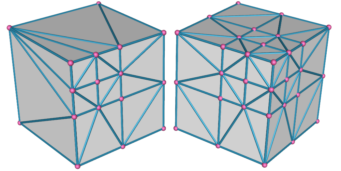
\includegraphics{VTKTextbook-48}\\
		\caption*{\texttt{Compatible tessellations.}}
	\end{minipage}
\end{figure}

\firstletter{I}n Chapter 4 we developed a pragmatic definition of the visualization process: mapping information into graphics primitives.
We saw how this mapping proceeds through one or more steps, each step transforming data from one form, or data representation, into another.
In this chapter we examine common data forms for visualization.
The goal is to familiarize you with these forms, so that you can visualize your own data using the tools and techniques provided in this text.

\section{Introduction}
To design representational schemes for data we need to know something about the data we might
encounter. We also need to keep in mind design goals, so that we can design efficient data structures
and access methods. The next two sections address these issues.

\subsection{Characterizing Visualization Data}
Since our aim is to visualize data, clearly we need to know something about the character of the
data. This knowledge will help us create useful data models and powerful visualization systems.

\section{Bibliographic Notes}

A variety of representation schemes have been proposed for each dataset type described here. These schemes vary depending on design goals. For example, even the simple volume representation has been implemented with other more complex schemes such as run-length encoding and octrees \cite{Bloomenthal88}. A description of more general representation schemes is available in \cite{Haber91}, the AVS field model \cite{AVS89}, and the compact cell structure \cite{Schroeder94}. An overview of dataset types can be found in \cite{Gelberg90}. Some structures for those mathematically oriented can be found in \cite{Brisson90} and \cite{Poluzzi93}. Haimes \cite{VISUAL3} describes an efficient data structure for unstructured grid visualization.

If you are interested in more details on finite element methods see the classic Zienkiewicz \cite{Zienkiewicz87} or \cite{Gallagher75}. Information about both finite difference and finite element methods is available in \cite{Lapidus82}.

\printbibliography


\section{Exercises}

\begin{enumerate}

\item Item 1

\item Item 2


\end{enumerate}